\documentclass[format=acmsmall, review=false, screen=true]{acmart}		% ICFP
%\documentclass[format=sigplan, review=true]{acmart}		% HASKELL SYMPOSIUM 
%\documentclass[format=sigconf, review=true]{acmart}		% IFL

\usepackage{float}
\usepackage{graphicx}
\usepackage{subcaption}
\usepackage{ifthen}
\usepackage{minted}
\usepackage{verbatim}

% Metadata Information
%% use defaults for review submission.
%\acmConference[HS18]{Haskell Symposium}{2018}{09}
%\acmYear{2018}
%\copyrightyear{2018}
\acmConference[IFL'18]{International Symposium on Implementation and Application of Functional Languages}{August 2019}{Lowell, MA, USA}
\acmYear{2019}
\copyrightyear{2019}
%\acmDOI{} % \acmDOI{10.1145/nnnnnnn.nnnnnnn}

% Copyright
%% use 'none' for review submission.
\setcopyright{none}
%\setcopyright{acmcopyright}	% = copyright transfer to ACM
%\setcopyright{acmlicensed} 		% = retaining copyright but granting ACM exclusive publication rights
%\setcopyright{rightsretained}  % = open access on payment of a fee
%\setcopyright{usgov}
%\setcopyright{usgovmixed}
%\setcopyright{cagov}
%\setcopyright{cagovmixed}

% TODO : get the data
% DOI
% \acmDOI{0000001.0000001}

% TODO: fill in
% Paper history
\received{May 2018}
%\received[revised]{March 2018}
%\received[accepted]{March 2018}

% Document starts
\begin{document}

\newminted[HaskellCode]{haskell}{fontsize=\footnotesize}

% Title portion. Note the short title for running heads
\title[Hands Off My Property!]{Hands Off My Property!}
\subtitle{The Potential Of Property-Based Testing In Agent-Based Simulation}

\author{Jonathan Thaler}
\orcid{https://orcid.org/0000-0001-8736-0479}
\email{jonathan.thaler@nottingham.ac.uk}
\affiliation{%
  \institution{University of Nottingham}
  \streetaddress{7301 Wollaton Rd}
  \city{Nottingham}
  \postcode{NG8 1BB}
  \country{United Kingdom}}

\begin{abstract}
This paper presents a new and complementary approach to unit-testing the implementation of agent-based simulations, called property-based testing which allows to test specifications of the implementation directly in code which is then tested using \textit{automated} test-data generation. We present two different models as case-studies in which we will show how to apply property-based testing to exploratory and explanatory agent-based models and what its limits are.

We conduct our implementations in the pure functional programming language Haskell, which is the origin of property-based testing. Also we show that simply by switching to such a language one gets rid of a large class of run-time bugs and is able to make stronger guarantees of correctness already at compile time without writing tests for some parts. Further, it makes isolated unit-tests quite easier.
\end{abstract}

%
% The code below should be generated by the tool at
% http://dl.acm.org/ccs.cfm
% Please copy and paste the code instead of the example below.
%
% TODO needs to be generated
%\begin{CCSXML}
%<ccs2012>
% <concept>
%  <concept_id>10010520.10010553.10010562</concept_id>
%  <concept_desc>Computer systems organization~Embedded systems</concept_desc>
%  <concept_significance>500</concept_significance>
% </concept>
% <concept>
%  <concept_id>10010520.10010575.10010755</concept_id>
%  <concept_desc>Computer systems organization~Redundancy</concept_desc>
%  <concept_significance>300</concept_significance>
% </concept>
% <concept>
%  <concept_id>10010520.10010553.10010554</concept_id>
%  <concept_desc>Computer systems organization~Robotics</concept_desc>
%  <concept_significance>100</concept_significance>
% </concept>
% <concept>
%  <concept_id>10003033.10003083.10003095</concept_id>
%  <concept_desc>Networks~Network reliability</concept_desc>
%  <concept_significance>100</concept_significance>
% </concept>
%</ccs2012>
%\end{CCSXML}
%
%\ccsdesc[500]{Computer systems organization~Embedded systems}
%\ccsdesc[300]{Computer systems organization~Redundancy}
%\ccsdesc{Computer systems organization~Robotics}
%\ccsdesc[100]{Networks~Network reliability}

%
% End generated code
%

\keywords{Agent-Based Simulation, Property-Based Testing, Model Checking, Haskell}

\maketitle

\section{Introduction}
There exists a large number of simulation packages which allow the convenient creation of System Dynamics simulations by straight-forward visual diagram creation. One simply creates stocks and flows, connects them, specifies the flow-rates and initial parameters and then runs the model. An example for such a visual diagram creation in the simulation package AnyLogic can be seen in Figure \ref{fig:sir_stockflow_diagram}.

\begin{figure}
	\centering
	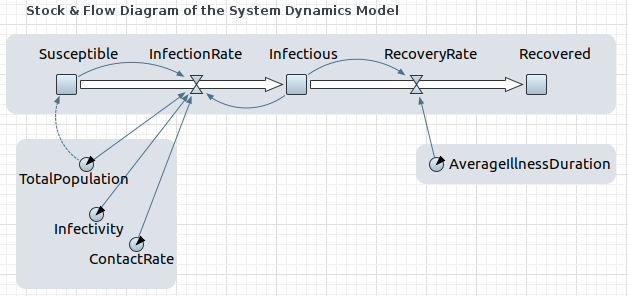
\includegraphics[width=.5\textwidth, angle=0]{./fig/SIR_SD_STOCKFLOW_DIAGRAMM.png}
	\caption{Visual System Dynamics Diagram of the SIR model in AnyLogic Personal Learning Edition 8.3.1.}
	\label{fig:sir_stockflow_diagram}
\end{figure}

Still, implementing System Dynamics directly in code is not as straight forward and involves numerical integration which can be quite tricky to get right. Thus, the aim of this paper is to look into how System Dynamics models can be implemented in code correctly without the use of a simulation package. We use the well known SIR model \cite{kermack_contribution_1927} from epidemiology to demonstrate our approach.

Our language of choice is Haskell because it emphasises a declarative programming style in which one describes \textit{what} instead of \textit{how} to compute. Further it allows to rule out interference with non-deterministic influences or side-effects already at compile-time. This is of fundamental importance for System Dynamics because it behaves completely deterministic and involves no stochastics or non-determinism whatsoever. Also, we make use of Functional Reactive Programming which allows to express continuous-time systems in a functional way. 

We show that by this approach we can arrive at correct-by-construction implementations of System Dynamic models. This means that the correctness of the code is obvious because we have closed the gap between the model specification and its implementation. Thus, the contribution of the paper is the demonstration of how to implement correct-by-construction System Dynamics simulations using Haskell and Functional Reactive Programming.

\section{Related Workd}
\label{sec:related}

% related works
% read all the papers peer has sent me
% https://www.atlassian.com/continuous-delivery/different-types-of-software-testing
%% TDD in ABS
Research on TDD of ABS is quite new and thus there exist relative few publications. The work \cite{collier_test-driven_2013} is the first to discusses how to apply the TDD approach to ABS, using unit-testing to verify the correctness of the implementation up to a certain level. They show how to implement unit-tests within the RePast Framework \cite{north_complex_2013} and make the important point that such a software need to be designed to be sufficiently modular otherwise testing becomes too cumbersome and involves too many parts. The paper \cite{asta_investigation_2014} discusses a similar approach to DES in the AnyLogic software toolkit. 

The paper \cite{onggo_test-driven_2016} proposes Test Driven Simulation Modelling (TDSM) which combines techniques from TDD to simulation modelling. The authors present a case study for maritime search-operations where they employ ABS. They emphasise that simulation modelling is an iterative process, where changes are made to existing parts, making a TDD approach to simulation modelling a good match. They present how to validate their model against analytical solutions from theory using unit-tests by running the whole simulation within a unit-test and then perform a statistical comparison against a formal specification. This approach will become of importance later on in our SIR case study.

The paper \cite{brambilla_property-driven_2012} propose property-driven design of robot swarms. They propose a top-down approach by specifying properties a swarm of robots should have from which a prescriptive model is created, which properties are verified using model checking. Then a simulation is implemented following this prescriptive and verified model after then the physical robots are implemented. The authors identify the main difficulty of implementing such a system that the engineer must \textit{"think at the collective-level, but develop at the individual-level}. It is arguably true that this also applies to implementing agent-based models and simulations where the same collective-individual separation exists from which emergent system behaviour of simulations emerges - this is the very foundation of the ABS methodology.

The paper \cite{gurcan_generic_2013} gives an in-depth and detailed overview over verification, validation and testing of agent-based models and simulations and proposes a generic framework for it. The authors present a generic UML class model for their framework which they then implement in the two ABS frameworks RePast and MASON. Both of them are implemented in Java and the authors provide a detailed description how their generic testing framework architecture works and how it utilises JUnit to run automated tests. To demonstrate their framework they provide also a case study of an agent-base simulation of synaptic connectivity where they provide an in-depth explanation of their levels of test together with code.

The review of the literature in the field gives the impression, that most research focuses on high-level validation and does not deal too much with verification on a technical, code-base level.

%% TDD in MAS
Although the work on TDD is scarce in ABS, there exists quite some research on applying TDD and unit-testing to multi-agent systems (MAS). Although MAS is a different discipline than ABS, the latter one has derived many technical concepts from the former one thus testing concepts applied to MAS might also be applicable to ABS. The paper \cite{nguyen_testing_2011} is a survey of testing in MAS. It distinguishes between unit tests which tests units that make up an agent, agent tests which test the combined functionality of units that make up an agent, integration tests which test the interaction of agents within an environment and observe emergent behaviour, system test which test the MAS as a system running at the target environment and acceptance test in which stakeholders verify that the software meets their goal. Although not all ABS simulations need acceptance and system tests, still this classification gives a good direction and can be directly transferred to ABS.  %Further the paper enumerates existing research and shows that some research is working on generating automated test input for agent level tests. 

%The paper \cite{tiryaki_sunit:_2007} discusses Test Driven Development in MAS and puts much emphasis on proposing agile processes to develop MAS software to handle complexity and continuously changing nature of requirements. The authors develop the SUNIT testing framework to implement unit-testing in an MAS environment.

\section{Pure Functional Programming}
\label{sec:background_fp}
To be able to understand the challenges of pure functional ABS as well as the solutions and concepts developed in this thesis, in this section we give a short introduction to functional programming, with an overview of its concepts and advanced features. As it is obviously beyond the focus of a thesis to give a full treatment of such a complex topic, we refer to additional literature and references for further discussions where appropriate.

Functional programming is called \textit{functional} because it makes functions the main concept of programming, promoting them to first-class citizens. This means that functions can be assigned to variables, they can be passed as arguments to other functions and they can be constructed as return values from functions. The roots of functional programming lie in Lambda Calculus which was first described by Alonzo Church \cite{church_unsolvable_1936}. This is a fundamentally different approach to computing than imperative programming (including established object-orientation), the roots of which lie in the Turing Machine \cite{turing_computable_1937}. Rather than describing \textit{how} something is computed as in the more operational approach of the Turing Machine, due to the more \textit{declarative} nature of Lambda Calculus, code in functional programming describes \textit{what} is computed.

In \cite{maclennan_functional_1990} the author defines functional programming as a methodology attributing the following properties to it: programming without the assignment-operator, allowing for higher levels of abstraction, allowing to develop executable specifications and prototype implementations, connected to computer science theory, performing algebraic reasoning. Further, the author makes the subtle distinction between \textit{applicative} and \textit{functional} programming. Applicative programming can be understood as applying values to functions where one deals with pure expressions. In those expressions the value is independent from the evaluation order, also known as referential transparency. This means that such functions have no side effects and thus the outcome of their execution does not depend on the history or context of the system. Additionally, inputs and effects to an operation are obvious from the written form.

Applicative programming is not necessarily unique to the functional programming paradigm but can be emulated in an imperative language like C as well. Functional programming is then defined by \cite{maclennan_functional_1990} as applicative programming with \textit{higher-order} functions. These are functions which operate themselves on functions: they can take functions as arguments, construct new functions and return them as values. This is in stark contrast to first-order functions, as used in applicative or imperative programming, which just operate on data alone. Higher-order functions allow the capturing of frequently recurring patterns in functional programming in the same way that imperative languages captured patterns like \texttt{goto}, \texttt{while-do}, \texttt{if-then-else}, \texttt{for}. Common patterns in functional programming are (amongst others) the \texttt{map}, \texttt{fold}, \texttt{zip} functions. So, functional programming is not really possible in the same way as in classic imperative languages like C, as it is not possible to construct new functions and return them as results from functions. Object-oriented languages like Java provide mechanisms allowing us to partially work around this limitation but are still far from \textit{pure} functional programming.

The equivalence in functional programming to the semicolon (;) operator of imperative programming, that allows us to compose imperative statements, is function composition. Function composition has no side effects, as opposed to the imperative semicolon operator, which simply composes destructive assignment statements executed after another, resulting in side effects.
At the heart of modern functional programming is monadic programming which is polymorphic function composition. One can implement a user-defined function composition by running code in between function composition - this code, of course, depends on the type of the Monad one runs in. This allows for emulating all kinds of effectful programming in an imperative style within a pure functional language (see Section \ref{sec:purity_sideeffects} below). Although it might seem strange following an imperative style in a pure functional language, some problems are inherently imperative in the way that computations need to be executed in a given sequence exhibiting some effects. In addition, a pure functional language needs to have some way to deal with effects, otherwise it would never be able to interact with the outside world and would be practically useless. The real benefit of monadic programming is that it is explicit about side effects and allows only effects which are fixed by the type of the Monad - the side effects which are possible are determined statically during compile time by the type system. Some general patterns can be extracted for example a \texttt{map}, \texttt{zip}, \texttt{fold} over Monads which results in effect-polymorphic behaviour. %this is the meaning when one says that a language is polymorphic in its side effects.

\subsection{Language of choice}
In our research we are using the \textit{pure} functional programming language Haskell. The paper \cite{hudak_history_2007} gives a comprehensive overview over the history of the language, how it developed and its features. The reasons for choosing Haskell are as follows:

\begin{itemize}
	\item Rich feature-set - it has all the fundamental concepts of the pure functional programming paradigm included, of which the most important ones are explained below. Moreover, Haskell has influenced a large number of languages, underlining its importance and influence in programming language design.
	
	\item Real-world applications - the strength of Haskell has been proven through a vast amount of highly diverse real-world applications \cite{hudak_history_2007, hudak_haskell_1994}. It is applicable to a number of real-world problems \cite{osullivan_real_2008} and has a large number of libraries available \cite{haskell_applications}.
	
	\item Modern - Haskell is constantly evolving through its community and adapts to keep up with the fast-paced changes in the field of computer science. Additionally, the community is the main source of high-quality libraries.
	
	\item Highly advanced type system - Haskell has a strong static type system, which catches all type errors at compile time and does not allow for bypassing the type system (unless \texttt{coerce} or other cheating functions like \texttt{unsafePerformIO} are used). In addition, Haskell is a \textit{pure} functional language and in our research it is absolutely paramount, that we focus on \textit{pure} functional ABS, which avoids any \texttt{IO} type under all circumstances. This property is enabled by the advanced type system and its strong static nature.
\end{itemize}

A highly compelling example motivating the benefits of pure functional programming is the report \cite{hudak_haskell_1994}. Where, in a prototyping contest of DARPA the Haskell prototype was by far the shortest, with 85 lines of code (LoC), as compared to the C++ solution with 1105 LoC. The remarkable thing is that the jury mistook the Haskell code as specification because its approach was to implement a small embedded domain specific language (EDSL) to solve the problem. This is a perfect proof as to how close an EDSL can get to a specification. When implementing an EDSL, one develops types and functions in a host language (embed) in a way where they can be combined. The combination of these primitives then looks like a language specific to a given domain. The ease of development of EDSLs in pure functional programming is also proof of the superior extensibility and composability of pure functional languages over object-orientation and is definitely one of its major strengths. The classic paper \cite{henderson_functional_1982} shows a wonderful way of constructing an EDSL to denotationally construct a picture reminiscent of the works of M.C.Escher. A major strength of developing an EDSL is that one can formally reason about it and do formal verification. A nice introduction about how to do reasoning in Haskell is given in \cite{hutton_tutorial_1999}.

For an excellent and widely used introduction to programming in Haskell we refer to \cite{hutton_programming_2016}. Other, more exhaustive books on learning Haskell are \cite{allen_haskell_2016, lipovaca_learn_2011}. For an introduction to programming with the Lambda-Calculus we can refer to \cite{michaelson_introduction_2011}. For a more general discussion of functional programming we refer to \cite{hudak_history_2007,hughes_why_1989,maclennan_functional_1990}.

\subsection{An Example}
Consider the factorial function in Haskell:
\begin{HaskellCode}
factorial :: Integer -> Integer
factorial 0 = 1
factorial n = n * factorial (n-1)
\end{HaskellCode}

When looking at this function, the following can be identified: 
\begin{enumerate}
	\item Declarative - describe \textit{what} the factorial function is, rather than how to compute it. This fact is supported by \textit{pattern matching} which allows providing multiple equations for the same function, matching on its input. 
	
	\item Immutable Data - in functional programming there are no mutable variables, after a variable is assigned, it cannot change its contents. This also means that there is no destructive assignment operator that can reassign values to a variable. To change values, recursion is employed.

	\item Recursion - the function calls itself with a structurally smaller argument and will eventually reach the base case of 0. Recursion is the very meat of functional programming because it is the only way to implement loops in this paradigm due to immutable data.
	
	\item Static Types - the first line indicates the name and the type of the function. In this case the function takes one Integer as input and returns an Integer as the output. Types are static in Haskell, which means that there can be no type errors at run time. For example it is not supported by this kind of type system to implicitly cast one type into another.

	\item Explicit Input and Output - all data which are required and produced by the function have to be explicitly passed in and out of it. No global mutable data exists whatsoever and data flow is always explicit.
	
	\item Referential Transparency - calling this function with the same argument will \textit{always} lead to the same result. Meaning one can replace this function by its value. Consequently, when implementing this function one cannot read from a file or open a connection to a server. This is also known as \textit{purity} and is indicated in Haskell in the types which means that it is also guaranteed by the compiler.
\end{enumerate}

It may seem that one runs into efficiency problems in Haskell when using algorithms which are implemented in imperative languages through mutable data, which allows in-place update of memory. The seminal work of \cite{okasaki_purely_1999} shows that when approaching this problem with a functional mindset, this issue will not necessarily be the case. The author presents functional data structures which are asymptotically as efficient as the best imperative implementations and discusses the estimation of the complexity of lazy programs.

\subsection{Purity and Side Effects}
\label{sec:purity_sideeffects}
One of the fundamental strengths of Haskell is its way of dealing with side effects in functions. A function with side effects has observable interactions with some state outside of its explicit scope. Therefore, its behaviour depends on the history of the system which means that it loses its referential transparency character, which makes understanding and debugging much harder. Possible examples of side effects are (amongst others): modifying a variable, awaiting an input from the keyboard, reading or writing to a file, opening a connection to a server, drawing random numbers.

Obviously, to write real-world programs which interact with the outside world requires side effects. Haskell allows for indicating in the \textit{type} of a function that it does, or does \textit{not} have side effects. What is more, there is a broad range of different effect types available, to restrict the possible effects a function can have to only the required type. This is checked by the compiler, which means that code which tries to read from a file in a function, when only allowing for drawing random numbers, will fail to compile.

A function without any side effect type is called \textit{pure}, and the \texttt{factorial} function discussed above is indeed pure. Below we give the \texttt{queryUser} function as an example of a function which is not pure. It constructs a computation, which when executed, asks the user for its user name and compares it with a given user configuration. In the event that the user name matches, it returns \texttt{True}, and \texttt{False} otherwise after printing a corresponding message. The effect type of the function is \texttt{IO}, which allows all kind of input-output related side effects like reading and writing a file, creating threads, writing to the standard output, reading from the keyboard, opening network connections and modifying mutable references.

\begin{HaskellCode}
queryUser :: String -> IO Bool
queryUser username = do
  -- print text to console
  putStr "Type in user-name: "
  -- wait for user-input
  str <- getLine
  -- check if input matches user-name
  if str == username
    then do
      putStrLn "Welcome!"			
      return True
    else do
      putStrLn "Wrong user-name!"
      return False
\end{HaskellCode}

What seems striking is that this looks very much like imperative code, which is no coincidence, but rather very much intentional. When we are dealing with side effects, ordering becomes important. Thus, Haskell introduced the so-called \textit{do} notation which emulates an imperative style of programming. Whereas, in imperative programming languages like C, instructions are chained or composed together using the semicolon (;) operator, in functional programming this is done using function composition. That is, feeding the output of a function directly into the next function. The machinery behind the \textit{do} notation does exactly this and desugars this imperative-style code into function compositions which run custom code between each line, depending on the type of effect the computation runs in. This approach of function composition with custom code in between each function allows to emulate a broad range of imperative-style effects, including the above-mentioned ones.

Although it might seem very restrictive at first, we get a number of benefits from making the type of effects we can use in a function explicit. First, we can restrict the side effects a function can have to a very specific type which is guaranteed at compile time. This means we can have much stronger guarantees about our program and the absence of potential errors immediately at compile time. Second, because running effects themselves is \textit{pure}, we can execute functions with effects in a very controlled way by making the context of the effect explicit in the parameters to the effect execution. This allows for a much easier approach to isolated testing because the history of the system is made explicit. 

\subsubsection{Monads}
Haskell implements its way of dealing with side effects using the concept of \textit{Monads}. It is important to understand that Monads are implemented directly in Haskell, which means that effects (with the exception of \texttt{IO} Monad) are implemented in terms of Haskell and not built into the runtime. To better understand how Haskell implements its concept of side effects with Monads, in this section, we briefly give an overview of what Monads are, how they are defined in Haskell and how they are used to facilitate effectful programming in a pure functional way. As this is a vast and complex topic, we can only scratch the surface here, consequently for a more technical, in-depth discussion we refer to \cite{jones_tackling_2002,moggi_computational_1989,wadler_essence_1992,wadler_monads_1995,wadler_how_1997}.

A Monad is an algebraic structure from the field of Category Theory. Moggi \cite{moggi_computational_1989} realised that Monads can be used to structure computation and later, Wadler \cite{wadler_monads_1995,wadler_how_1997} realised that Monads can be used as a way to achieve effectful computation in pure functional programming. 

Without going into the mathematical details, we give the definition of Monads in Haskell. Informally speaking, in Haskell, a Monad is both an Applicative and a Functor, which provides the operation \textit{return} and \textit{bind}. The according type class is:

\begin{HaskellCode}
-- Monad type class
-- Applicative and Functor omitted for clarity
class Applicative m => Monad m where
  return :: a -> m a
  -- bind, in Haskell >>= is used
  (>>=) :: m a -> (a -> m b) -> m b
\end{HaskellCode}

%-- Applicative type class
%-- Allows composing functions which map over values with structure.
%class Functor f => Applicative f where
%  pure  :: a -> f a
%  (<*>) :: f (a -> b) -> f a -> f b
%
%-- Functor type class
%-- Allows mapping between values with some structure.
%class Functor f where
%  fmap :: (a -> b) -> f a -> f b

\texttt{return} lifts a pure value into a Monad. \texttt{bind (>>=)} allows to sequence computations, feeding the output \texttt{a} of the first computation into a continuation, which returns a new computation in the same Monad \texttt{m} but with a possibly different return type \texttt{b}. Interestingly, with this interface it becomes possible to implement a wide range of pure, deterministic effects. As already mentioned above, in between lines of the \textit{do} notation runs custom code. This is achieved which the \texttt{bind (>>=)} method. The \texttt{return}, also seen above in the example, lifts a pure value, in the example a \texttt{Boolean} value, into a monadic value.

Obviously, the Monad type class only defines the interface required for a Monad but no actual implementations. There are a number of different Monad implementations, providing different types of side effects:

\begin{itemize}
	\item \texttt{Reader} uses partial function application to implement reading from an environment;
	\item \texttt{Writer} uses a monoid type to implement writing to a \textit{monoid} environment;
	\item \texttt{State} uses functions and closures to implement reading and writing shared state of a given type;
	\item \texttt{Rand} uses a \texttt{State} Monad to implement a random number stream;
	\item \texttt{[] (List)} forms also a Monad and implements non-deterministic programming.
\end{itemize}

To better understand how a Monad is implemented, we show the implementation of the \texttt{Maybe} Monad, which allows programming with failure. The \texttt{Maybe} type itself is straightforward and provides some kind of optional value, where a computation can either return \texttt{Just} some value or \texttt{Nothing}:

\begin{HaskellCode}
data Maybe a = Nothing | Just a
\end{HaskellCode}

Interestingly, \texttt{Maybe} forms a Monad. It allows us to write imperative-style code with the option of failure but saves us from handling each failure individually. Here is the implementation:

\begin{HaskellCode}
-- Instance of Maybe Monad.
-- Type definitions of methods provided for clarification
instance Monad Maybe where
  return :: a -> Maybe a
  return = Just
  
  (>>=) :: Maybe a -> (a -> Maybe b) -> Maybe b
  (>>=) Nothing _  = Nothing
  (>>=) (Just a) f = f a 
\end{HaskellCode}

\texttt{return} simply lifts a pure value \texttt{a} into a \texttt{Just} value, applying the data constructor \texttt{Just}. \texttt{bind (>>=)} performs case analysis: if \texttt{Maybe a} is Nothing, the it will propagate \texttt{Nothing}, otherwise it will use \texttt{a} with the continuation \texttt{f}, to return the next computation \texttt{Maybe b}.

\medskip

It is important to understand that the code fragments of effectful computations are in fact  made up of enclosing lambda expressions, with the \textit{do} notation being a syntactic sugared version. Thus functions which have an effect in their type can be seen as \textit{pure} functions, which are referentially transparent and return such a fragment. This fragment, often called \textit{action}, results in an effect and a result when executed. We have to distinguish between the execution of pure effects like \texttt{Rand}, \texttt{Read}, \texttt{Write}, \texttt{State} and the impure effect of \texttt{IO}. Pure effects are executed using special runner functions. They take an action together with one or more initial values defining the history or context of the effect - for example, an initial value for the \texttt{State} or the read-only value of the \texttt{Reader} - and then run the action returning their its value. Consequently, these pure effects can be executed in a referential transparent and completely controlled way.

However, the impure \texttt{IO} effect works differently. There is no dedicated \texttt{IO} execution function that exists, but it can only be executed from within the root \texttt{IO} action. This root action emanates from the \texttt{main :: IO ()} function of each Haskell program. As a result, \texttt{IO} actions can only be run within an enclosing \texttt{IO} action. The main \texttt{IO} action is then ultimately being executed by the Haskell runtime, which is linked against the executable. The reason for that is that if we did have a way of executing \texttt{IO} actions within pure code, we would lose all guarantees about referential transparency. The function \texttt{unsafePerformIO :: IO a $\rightarrow$ a}, exists, which allows for executing an \texttt{IO} action within a pure function, but its use is very limited and highly discouraged. Throughout this thesis and in all our code, we have avoided the use of this function at all costs. Consequently it is not used anywhere in this work, as avoiding \texttt{IO} is the very meaning of \textit{purity} and \textit{pure} functional programming.

\subsubsection{Stacking Effects}
\label{sec:back_transformers}
Often it is necessary to have multiple effects available for use. For example, if we want to manipulate a global state, write to some logging mechanism and need to be able to draw random numbers. Although Monads share a common interface and properties, it is not possible to compose Monads in general. Because each Monad has different internals and semantics, without knowing one of the two Monad to compose, it is not possible to combine them in general. Therefore, to combine two Monads, one is kept polymorphic, while the other one is known. The way this is achieved in Haskell is by using Monad Transformers \cite{allen_haskell_2016, jones_functional_1995, jones_tackling_2002}. Haskell provides the two libraries \textit{mtl} and \textit{transformers} for this, with \textit{transformers} being the older library but \textit{mtl} building on \textit{transformers}, additionally allowing for overloading functions with monadic type classes as explained below. In our approach we use both without making a distinction.

A Transformer consists of a type constructor which takes an existing Monad and returns a Monad as result. It also needs to provide implementations of both the \texttt{return} and \texttt{bind} monadic operations. Also, it needs to provide an operation \texttt{lift :: Monad m $\Rightarrow$ m a $\rightarrow$ t m a}, which allows to execute ('lift') a monadic operation \texttt{m a} from the existing Monad \texttt{m} within (into) the Transformer \texttt{t}. Therefore a Transformer is always a Monad itself, which allows for the stacking of multiple Monads or Transformers on top of each other. The stack is closed by using a non-Transformer Monad. All non-Transformer Monads are actually Transformers with the \texttt{Identity} Monad as the type parameter.

Implementing Transformers can get tricky, but as a relatively simple example, we show the implementation of the \texttt{MaybeT} Transformer from the \textit{transformers} library. The \texttt{MaybeT} is a Transformer which allows the inclusion of the \texttt{Maybe} Monad into a Transformer stack, to enable effectful computations which might fail. First, we provide the type constructor for the Transformer, which is a wrapper around the \texttt{Maybe} type, adding an arbitrary Monad \texttt{m}:

\begin{HaskellCode}
newtype MaybeT m a = MaybeT { runMaybeT :: m (Maybe a) }
\end{HaskellCode}

Then, we provide the the implementation \cite{allen_haskell_2016} of the \texttt{Monad} instance for the \texttt{MaybeT} type. Consequently, this makes \texttt{MaybeT} a Monad:

\begin{HaskellCode}
-- Instance of MaybeT Monad.
-- Type definitions of methods provided for clarification
instance (Monad m) => Monad (MaybeT m) where
  return :: a -> MaybeT a
  return = MaybeT . return . Just

  (>>=) :: MaybeT m a -> (a -> MaybeT m b) -> MaybeT m b
  (>>=) (MaybeT ma) f = MaybeT (do 
      v <- ma
      case v of
          Nothing -> return Nothing
          Just y  -> runMaybeT (f y))
\end{HaskellCode}

\texttt{return} puts the value \texttt{a} into \texttt{Just}, then lifts the \texttt{Maybe} value into the polymorphic Monad \texttt{m} and constructs a \texttt{MaybeT}. \texttt{bind (>>=)} is a bit more complex. It starts by constructing a \texttt{MaybeT} which first executes the polymorphic monadic action \texttt{ma}, resulting in a \texttt{Maybe} result. Then it performs a case analysis over the \texttt{Maybe} result. In case it is \texttt{Nothing}, it simply returns \texttt{Nothing} lifted into the polymorphic Monad \texttt{m}. In case it is \texttt{Just}, it applies the continuation \texttt{f} to get the new \texttt{MaybeT m b} value with which to construct the resulting \texttt{MaybeT}.

Finally, we provide the implementation of the \texttt{lift} operator:
 
\begin{HaskellCode}
lift :: m a -> MaybeT m a
lift = MaybeT . (liftM Just)

liftM :: Monad m => (a -> b) -> m a -> m b
\end{HaskellCode}

\texttt{lift} simply packs the value \texttt{a} into the \texttt{MaybeT m a}. It does it by using \texttt{liftM} to lift the pure data constructor \texttt{Just} into the polymorphic Monad \texttt{m}, and then constructing a \texttt{MaybeT}. Let's look at how we can define the type of a function which has multiple effects available:

\begin{HaskellCode}
data SimState = SimState { simStateAgents :: [SimAgent] ... }

simulationCore :: RandomGen g 
               => Time
               -> StateT SimState (WriterT [String] (Rand g)) SimOut
simulationCore t = do
  -- get the agents from the simulation state 
  -- encapsulated in StateT SimState
  as <- gets simStateAgents
  -- writing a logging output to the WriterT [String]
  -- here we need 1 lift 
  lift (tell ["Next step " ++ show t])
  -- shuffle agents by running the MonadRandom action using the
  -- Rand Monad, need 2 lifts as it is the innermost monad
  asShuf <- lift $ lift $ randomShuffle as
  -- construct return value
  return (SimOut { ... })
  
randomShuffle :: MonadRandom m => [a] -> m [a]
\end{HaskellCode}

The Monad stack consists of three effects. The first and \textit{outermost} effect is \texttt{StateT} with \texttt{SimState} as the internal state. As it is the outermost effect, no \texttt{lift} is required to access it. \texttt{WriterT} with \texttt{[String]} as the logging facility is a parameter to the \texttt{StateT} Transformer, making it the second effect in the stack, thus it requires one \texttt{lift}. The stack is closed using the \texttt{Rand} Monad, which is the \textit{innermost} effect, requiring two \texttt{lifts} to access it. As a result, in a Transformer stack, one needs to \textit{lift into} the stack, which means that although it is constructed inside to outside (\texttt{Rand} $\rightarrow$ \texttt{WriterT} $\rightarrow$ \texttt{StateT}) it is lifted from outside to inside (\texttt{StateT} $\rightarrow$ \texttt{WriterT} $\rightarrow$ \texttt{Rand}).

Executing a Monad Transformer stack works by using various monadic runner functions, which execute a Transformer layer with a given context as is shown in the example of section \ref{sec:back_msf} below. As with lifting, a Monad Transformer stack is evaluated from outside to inside (\texttt{StateT} $\rightarrow$ \texttt{WriterT} $\rightarrow$ \texttt{Rand}).

The function \texttt{randomShuffle} is overloaded, having the \texttt{MonadRandom} type class in its type constraints. This indicates that it is a monadic action where \texttt{m} is of type \texttt{MonadRandom}, which supports the same functionality as \texttt{Rand}. This is the major benefit mtl provides, often resulting in much cleaner function types, which do not require fixing the order of the Monads in the stack. Another benefit is that we do not need lifts anymore.The drawback is that we cannot have multiple Monads of the same type, which would be still possible in a fully qualified Monad stack. The benefits become particularly clear when more than one effect is required. For example, we can write the type of \texttt{simulationCore} as:

\begin{HaskellCode}
simulationCore :: (MonadState SimState m, MonadWriter [String] m, MonadRandom m) 
               => Time -> m SimOut
\end{HaskellCode}

A note on the commutativity of Monad Transformers: because we are stacking effects on top of each other, subsequent effects can change the final outcome, depending on their position within the stack - this is called commutativity of Monads. All the Monads in the example above commute. This means it does not matter where they are positioned in the stack, the outcome will be the same. An exception to this is the \texttt{MaybeT} Transformer, as shown above. As can be seen in the implementation, when failure occurs, subsequent effects will not be applied any more, making \texttt{MaybeT} non-commutative. Consider the following examples:

\begin{HaskellCode}
-- evaluates to: Just "Haskell" / Just 1
stateWithMaybe :: StateT Int Maybe String
stateWithMaybe = do
  modify (+1)
  return "Haskell"

-- evaluates always to Nothing
stateWithMaybeNothing :: StateT Int Maybe String
stateWithMaybeNothing = do
  modify (+1)
  lift Nothing

-- evaluates to (Just "Haskell",1)
maybeWithState :: MaybeT (State Int) String
maybeWithState = do
  lift $ modify (+1)
  return "Haskell"

-- evaluates to (Nothing,1)
maybeWithStateFail :: MaybeT (State Int) String
maybeWithStateFail = do
  lift $ modify (+1)
  fail "Some Failure"
\end{HaskellCode}

Depending on whether we want the \texttt{String} returned by the computation or the \texttt{Int} of the \texttt{StateT}, \texttt{stateWithMaybe} evaluates always to some \texttt{Just} value. However, \texttt{stateWithMaybeNothing} \textit{always} evaluates to \texttt{Nothing}, discharging the \texttt{Int} state of the \texttt{StateT}.

\texttt{maybeWithState} always evaluates to \texttt{(Just "Haskell",1)}: it returns \textit{both} the final value of the \texttt{State} \textit{and} the \texttt{String} returned by the computation. This makes it possible that \texttt{maybeWithStateFail} fails, therefore returning no \texttt{String} but still retaining the state of the \texttt{State} effect.

\subsection{Functional Reactive Programming}
\label{sec:back_frp}
Functional Reactive Programming (FRP) is a way to implement systems with continuous and discrete time semantics in pure functional languages. There are many different approaches and implementations but, in this thesis, \textit{Arrowized} FRP \cite{hughes_generalising_2000, hughes_programming_2005} as implemented in the library Yampa \cite{courtney_yampa_2003,hudak_arrows_2003,nilsson_functional_2002} and Dunai \cite{perez_functional_2016} (see below) is used.

The central concept in Arrowized FRP is the signal function (SF), which can be understood as a \textit{process over time} which maps an input- to an output signal. A signal can be understood as a value which varies over time. Therefore, signal functions have an awareness of the passing of time by having access to $\Delta t$ which are positive time steps, the system is sampled with:

\begin{flalign*}
Signal \, \alpha \approx Time \rightarrow \alpha \\
SF \, \alpha \, \beta \approx Signal \, \alpha \rightarrow Signal \, \beta 
\end{flalign*}

Yampa provides a number of combinators for expressing time semantics, events and state changes of the system. They allow to change system behaviour in case of events, run signal functions and generate stochastic events and random-number streams. Below, the relevant combinators and concepts used throughout the thesis are discussed briefly. For a more in-depth discussion we refer to \cite{courtney_yampa_2003, hudak_arrows_2003, nilsson_functional_2002} in the reference section.

\paragraph{Event}
An event in FRP is an occurrence at a specific point in time, which has no duration. An example of such an event would be the recovery of an infected agent. Yampa represents events through the \texttt{Event} type, which is programmatically equivalent to the \texttt{Maybe} type. 

\paragraph{Dynamic behaviour}
To change the behaviour of a signal function at an occurrence of an event during run time, (amongst others) the combinator \texttt{switch :: SF a (b, Event c) $\rightarrow$ (c $\rightarrow$ SF a b) $\rightarrow$ SF a b} is used. It takes a signal function, which is run until it generates an event. When this event occurs, the function in the second argument is evaluated, which receives the data of the event and has to return the new signal function. This new signal function will then replace the previous one. The semantics of \texttt{switch} are that the signal function, into which is switched, is also executed at the time of switching.

\paragraph{Randomness}
In ABS, often there is the need to generate stochastic events, which occur based on a certain distribution. Yampa provides the combinator \texttt{occasionally :: RandomGen g $\Rightarrow$ g $\rightarrow$ Time $\rightarrow$ b $\rightarrow$ SF a (Event b)} for this. It takes a random-number generator, a rate and a value the stochastic event will carry. It generates events on average with the given rate, following the exponential distribution. At most, one event will be generated and no backlog is kept. This means that when this function is not sampled with a sufficiently high frequency, depending on the rate, it will lose events.

Yampa also provides the combinator \texttt{noise :: (RandomGen g, Random b) $\Rightarrow$ g $\rightarrow$ SF a b}, which generates a stream of noise by returning a random number in the default range for the type \texttt{b}, following the uniform distribution.

\paragraph{Running signal functions}
To run a signal function Yampa provides the function \texttt{embed :: SF a b $\rightarrow$ (a, [(DTime, Maybe a)]) $\rightarrow$ [b]}, which allows for running an SF for a given number of steps. Where, in each step one provides the $\Delta t$ and an input \texttt{a}. The function then returns the output of the signal function for each step. The input is optional, indicated by \texttt{Maybe}. In the first step at $t = 0$, the initial \texttt{a} is applied and whenever the input is \texttt{Nothing} in subsequent steps, the last \texttt{a} which was not \texttt{Nothing} is reused.

\subsection{Arrowized programming}
Yampa's signal functions are Arrows, requiring us to program with Arrows. Arrows are a generalisation of Monads, which in addition to the already familiar parameterisation over the output type, allow parameterisation over their input type as well \cite{hughes_generalising_2000, hughes_programming_2005}. For a clearer understanding, we show how Arrows are defined in terms of Haskell \cite{arrows_haskell}:

\begin{HaskellCode}
class Arrow a where
  -- Each function may be treated as a computation.  
  arr :: (b -> c) -> a b c
  
  -- A computation applied to part of the input, 
  -- with the rest copied through to the output.
  first :: a b c -> a (b,d) (c,d)
  
  -- Computations may be composed, by connecting 
  -- the output of the first to the input of the second.
  (>>>) :: a b c -> a c d -> a b d
\end{HaskellCode}

It is clear to see in the type definitions, that each method also parametrises over the input type. As a simple example for an Arrow instance we provide the implementation of an Arrow for pure function computations:

\begin{HaskellCode}
newtype Func a b = Func { runFunc :: (a -> b) }

-- Instance of pure function computations as Arrow.
-- Type definitions of methods provided for clarification
instance Arrow Func where
  arr :: Func a b
  arr f = Func f

  first :: Func b c -> Func (b, d) (c, d)
  first (Func f) = Func (mapFst f)
    where
      mapFst g (a,b) = (g a, b)
    
  (>>>) :: Func b c -> Func c d -> Func b d
  (>>>) (Func f) (Func g) = Func (g . f)
\end{HaskellCode}

In general, Arrows can be understood to be computations that represent processes, which take an input of a specific type, process it and output a value of a given type. This is also reflected in the types of the \texttt{Arrow} type class and the example above: we are dealing with functions and not individual arguments, as in the case of Monads. The concept of processes, which signal functions indeed are, maps naturally to Arrows which is the reason why Yampa is using them to represent their signal functions.

There exists a number of Arrow combinators, which allow arrowized programming in a point-free style but due to lack of space we will not discuss them here. Instead we make use of Paterson's \textit{do} notation for arrows \cite{paterson_new_2001}, which makes the code more readable as it allows us to program with points.

To show how arrowized programming works, we implement a simple signal function, which calculates the acceleration of a falling mass on its vertical axis as an example \cite{perez_testing_2017}.

\begin{HaskellCode}
fallingMass :: Double -> Double -> SF () Double
fallingMass p0 v0 = proc _ -> do
  v <- arr (+v0) <<< integral -< (-9.8)
  p <- arr (+p0) <<< integral -< v
  returnA -< p
\end{HaskellCode}

To create an Arrow, the \texttt{proc} keyword is used, which binds a variable after which the \texttt{do} of Patersons \textit{do} notation \cite{paterson_new_2001} follows. Using the signal function \texttt{integral :: SF v v} of Yampa, which integrates the input value over time using the rectangle rule, we calculate the current velocity and the position based on the initial position \texttt{p0} and velocity \texttt{v0}. The \texttt{<<<} is one of the Arrow combinators, which composes two Arrow computations and \texttt{arr} simply lifts a pure function into an Arrow. To pass an input to an Arrow, \texttt{-<} is used and \texttt{<-} is used to bind the result of an Arrow computation to a variable. Finally to return a value from an Arrow, \texttt{returnA} is used.

\subsection{Monadic Stream Functions}
\label{sec:back_msf}
Monadic Stream Functions (MSF) are a generalisation of Yampa's signal functions but they have additional combinators to control and stack side effects. An MSF is a polymorphic type and an evaluation function, which applies an MSF to an input and returns an output and a continuation, both in a monadic context \cite{perez_extensible_2017,perez_functional_2016}:
\begin{HaskellCode}
newtype MSF m a b = MSF {unMSF :: MSF m a b -> a -> m (b, MSF m a b)}
\end{HaskellCode}

An MSF is also an Arrow, which means we can apply arrowized programming with Patersons \textit{do} notation as well. MSFs are implemented in Dunai, which is available on Hackage \cite{dunai_library}. Dunai allows for the application of monadic transformations by means of combinators like \texttt{arrM :: Monad m $\Rightarrow$ (a $\rightarrow$ m b) $\rightarrow$ MSF m a b} and \texttt{arrM\_ :: Monad m $\Rightarrow$ m b $\rightarrow$ MSF m a b}. A part of the library Dunai is BearRiver, a wrapper, which reimplements Yampa on top of Dunai. This wrapper enables one to run arbitrary monadic computations in a signal function. BearRiver simply adds a type parameter \texttt{m} to each \texttt{SF}, which indicates the monadic context in which this signal function runs.

To show how arrowized programming with MSFs works, we extend the falling mass example from above to incorporate effects. In this (artificial) example we assume that in each step we want to accelerate our velocity \texttt{v} not by the gravity constant anymore but by a random number in the range of 0 to 9.81. Moreover, we want to count the number of steps it takes us to hit the floor, that is, when the position \texttt{p} is less than 0. Additionally, when hitting the floor we want to print a debug message to the console with the velocity, by which the mass has hit the floor and how many steps it took.

We define a corresponding Monad stack with \texttt{IO} as the innermost Monad to print to the console, followed by a \texttt{RandT} Transformer for drawing random numbers, and finally, a \texttt{StateT} Transformer as the outermost Monad, to count the number of steps we compute. We can access the monadic functions using \texttt{arrM} in case we need to pass an argument, and \texttt{\_arrM}, in case no argument to the monadic function is needed:

\begin{HaskellCode}
type FallingMassStack g = StateT Int (RandT g IO)
type FallingMassMSF g   = SF (FallingMassStack g) () Double

fallingMassMSF :: RandomGen g => Double -> Double -> FallingMassMSF g
fallingMassMSF v0 p0 = proc _ -> do
  -- drawing random number for our gravity range
  r <- arrM_ (lift $ lift $ getRandomR (0, 9.81)) -< ()
  v <- arr (+v0) <<< integral -< (-r)
  p <- arr (+p0) <<< integral -< v
  -- count steps
  arrM_ (lift (modify (+1))) -< ()
  if p > 0
    then returnA -< p
    -- we have hit the floor
    else do
      -- get number of steps
      s <- arrM_ (lift get) -< ()
      -- write to console
      arrM (liftIO . putStrLn) -< "hit floor with v " ++ show v ++ 
                                  " after " ++ show s ++ " steps"
      returnA -< p
\end{HaskellCode}

To run the \texttt{fallingMassMSF} function until it hits the floor we proceed as follows:

\begin{HaskellCode}
runMSF :: RandomGen g => g -> Int -> FallingMassMSF g -> IO ()
runMSF g s msf = do
  let msfReaderT = unMSF msf ()
      msfStateT  = runReaderT msfReaderT 0.1 -- sampling with time delta of 0.1
      msfRandT   = runStateT msfStateT s
      msfIO      = runRandT msfRandT g
  (((p, msf'), s'), g') <- msfIO
  when (p > 0) (runMSF g' s' msf')
\end{HaskellCode}

Dunai does not know about time in MSF, which is exactly what BearRiver builds on top. It does so by adding a \texttt{ReaderT Double}, which carries the $\Delta t$. This is the reason why we need one extra lift for accessing \texttt{StateT} and \texttt{RandT}. Thus, \texttt{unMSF} returns a computation in the \texttt{ReaderT Double} Monad, which we need to peel away using \texttt{runReaderT}. This action then results in a \texttt{StateT Int} computation, which we evaluate by using \texttt{runStateT} and the current number of steps as state. This then results in another monadic computation of \texttt{RandT} Monad, which we evaluate using \texttt{runRandT}. This finally returns an \texttt{IO} computation, which we simply evaluate to arrive at the final result.

As explained in the previous section \ref{sec:back_transformers}, this example shows how a Monad Transformer stack is lifted and evaluated from outside to inside (\texttt{ReaderT} $\rightarrow$ \texttt{StateT} $\rightarrow$ \texttt{RandT} $\rightarrow$ \texttt{IO}) but constructed inside to outside (\texttt{IO} $\rightarrow$ \texttt{RandT} $\rightarrow$ \texttt{StateT} $\rightarrow$ \texttt{ReaderT}).

\section{Property-Based Testing}
\label{sec:proptesting}

Property-based testing allows to formulate \textit{functional specifications} in code which then a property-based testing library tries to falsify by \textit{automatically} generating test-data, covering as many cases as possible. When a case is found for which the property fails, the library then reduces the test-data to its simplest form for which the test still fails e.g. shrinking a list to a smaller size. It is clear to see that this kind of testing is especially suited to ABS, because we can formulate specifications, meaning we describe \textit{what} to test instead of \textit{how} to test. Also the deductive nature of falsification in property-based testing suits very well the constructive and exploratory nature of ABS. Further, the automatic test-generation can make testing of large scenarios in ABS, which is almost always stochastic by nature, feasible as it does not require the programmer to specify all test-cases by hand, as is required in traditional unit-tests.

Property-based testing was invented by the authors of \cite{claessen_quickcheck_2000,claessen_testing_2002} in which they present the QuickCheck library in Haskell, which tries to falsify the specifications by \textit{randomly} sampling the space. We argue, that the stochastic sampling nature of this approach is particularly well suited to ABS, because it is itself almost always driven by stochastic events and randomness in the agents behaviour, thus this correlation should make it straight-forward to map ABS to property-testing. A challenge when using QuickCheck is to write \textit{custom} test-data generators for agents and the environment, which cover the space sufficiently enough to not miss out on important test-cases. According to the authors of QuickCheck \textit{"The major limitation is that there is no measurement of test coverage."} \cite{claessen_quickcheck_2000}. QuickCheck provides help to report the distribution of test-cases but still it could be the case that simple test-cases which would fail are never tested because of the stochastic nature of QuickCheck.

To give a rough idea on how property-based testing works in Haskell, we give a few examples of properties on lists, which are directly expressed as functions in Haskell. Such a function has to return a \textit{Bool}, which indicates \textit{True} in case the test succeeds or \textit{False} if not and can take input arguments which data is automatically generated by QuickCheck. Note that the first line of each function defines its name, its inputs (\textit{[Int]} is a list of integers) and the output which is the last type (\textit{Bool}). Note that the \textit{(++)} operator concatenates two lists, \textit{reverse} simply reverses a list.

\begin{HaskellCode}
-- concatenation operator (++) is associative
append_associative :: [Int] -> [Int] -> [Int] -> Bool
append_associative xs ys zs = (xs ++ ys) ++ zs == xs ++ (ys ++ zs)

-- reverse is distributive over concatenation (++)
-- xs and ys need to be swapped on the right-hand side!
reverse_distributive :: [Int] -> [Int] -> Bool
reverse_distributive xs ys = reverse (xs ++ ys) == reverse ys ++ reverse xs

-- the reverse of a reversed list is the original list
reverse_reverse :: [Int] -> Bool
reverse_reverse xs = reverse (reverse xs) == xs
\end{HaskellCode}

% POTENTIAL FOR SHORTENING
As a remedy for the potential sampling difficulties of QuickCheck, there exists also a deterministic property-testing library called SmallCheck \cite{runciman_smallcheck_2008}, which instead of randomly sampling the test-space, enumerates test-cases exhaustively up to some depth. It is based on two observations, derived from model-checking, that (1) \textit{"If a program fails to meet its specification in some cases, it almost always fails in some simple case"} and (2) \textit{"If a program does not fail in any simple case, it hardly ever fails in any case} \cite{runciman_smallcheck_2008}. This non-stochastic approach to property-based testing might be a complementary addition in some cases, where the tests are of non-stochastic nature with a search-space which is too large to implement manually by unit-tests but is relatively easy and small enough to enumerate exhaustively. The main difficulty and weakness of using SmallCheck is to reduce the dimensionality of the test-case depth search to prevent combinatorial explosion, which would lead to an exponential number of cases. Thus, one can see QuickCheck and SmallCheck as complementary instead of in opposition to each other.
% POTENTIAL FOR SHORTENING
Note that in this paper we only use QuickCheck due to the match of ABS stochastic nature and the random test generation. Also note that we regard property-based testing as \textit{complementary} to unit-tests and not in opposition - we see it as an addition in the TDD process of developing an ABS.

\section{Pure Functional ABS}
TODO: introduce the general concepts of pure functional ABS and what the benefits and drawbacks are in the context of debugging and correctness. 
TODO: List of Common Bugs and Programming Practices to avoid them \cite{vipindeep_list_2005}

We argue that due to its fundamental different nature, the functional programming paradigm can overcome some fundamental problems of the established object-oriented approach to ABS. Note that we don't claim that it will solve all the problems and that the Gintis failure wouldn't have happened but we argue that it makes making mistakes much harder, resulting in simulations which are more likely to be correct.

We have investigated the concepts of \textbf{\textit{how}} to do agent-based simulation using the functional programming paradigm, as in the language Haskell, which is described in the paper in Appendix \ref{app:pfe}. The approach we developed is based on Functional Reactive Programming which allows to express discrete- and continuous-time systems in functional programming. Following the conclusions of the paper, we got the following benefits, supporting directly our initial hypothesis and our claims above, giving good reasons \textbf{\textit{why}} to do ABS in a functional way:

\begin{enumerate}
	\item Run-Time robustness by compile-time guarantees - by expressing stronger guarantees already at compile-time we can restrict the classes of bugs which occur at run-time by a substantial amount due to Haskell's strong and static type system.  This implies the lack of dynamic types and dynamic casts \footnote{Note that there exist casts between different numerical types but they are all safe and can never lead to errors at run-time.} which removes a substantial source of bugs.  Note that we can still have run-time bugs in Haskell when our functions are partial.
	\item Purity - By being explicit and polymorphic in the types about side-effects and the ability to handle side-effects explicitly in a controlled way allows to rule out non-deterministic side-effects which guarantees reproducibility due to guaranteed same initial conditions and deterministic computation. Also by being explicit about side-effects e.g. Random-Numbers and State makes it easier to verify and test.
	\item Explicit Data-Flow and Immutable Data - All data must be explicitly passed to functions thus we can rule out implicit data-dependencies because we are excluding IO. This makes reasoning of data-dependencies and data-flow much easier as compared to traditional object-oriented approaches which utilize pointers or references.
	\item Declarative - describing \textit{what} a system is, instead of \textit{how} (imperative) it works. In this way it should be easier to reason about a system and its (expected) behaviour because it is more natural to reason about the behaviour of a system instead of thinking of abstract operational details.
	\item Concurrency and parallelism - due to its pure and 'stateless' nature, functional programming is extremely well suited for massively large-scale applications as it allows adding parallelism without any side-effects and provides very powerful and convenient facilities for concurrent programming. We have explored this more in-depth in Chapter \ref{chap:stm}.
\end{enumerate}

In general, Types guide us in program construction by restricting the operations we can perform on the data. This means that by choosing types this reveals already a lot of our program and data and prevents us from making mistakes e.g. interpreting some binary data as text instead of a number. In strongly statically typed languages the types can do this already at compile-time which allows to rule out certain bugs already at compile-time. In general, we can say that for all bugs which can be ruled out at compile-time, we don't need to write property- or unit-tests, because those bugs cannot - per definition - occur at run-time, so it won't make sense to test their absence at run-time. Also, as Dijkstra famously put it: "Testing shows the presence, not the absence of bugs" - thus by induction we can say that compile-time guarantees save us from a potentially infinite amount of testing.

In general it is well established, that pure functional programming as in Haskell, allows to express much stronger guarantees about the correctness of a program \textit{already at compile-time}. This is in fundamental contrast to imperative object-oriented languages like Java or Python where only primitive guarantees about types - mostly relationships between type-hierarchies - can be expressed at compile-time which directly implies that one needs to perform much more testing (user testing or unit-testing) at \textit{run-time} to check whether the model is sufficiently correct. Thus guaranteeing properties already at compile-time frees us from writing unit-tests which cover these cases or test them at run time because they are \textit{guaranteed to be correct under all circumstances, for all inputs}.

In this regards we see pure functional programming as truly superior to the traditional object oriented approaches: they lead to implementations of models which are more likely correct because we can express more guarantees already at compile-time which directly leads to less bugs which directly increases the probability of the software being a correct implementation of the model. Having established this was only the first step in our paper in Appendix \ref{app:pfe}. 

Although pure functional ABS as in Haskell allows us to leverage on the concepts of functional and its benefits (and drawbacks) we still rely heavily on (property-based) testing to ensure correctness of a simulation because our approach still can have run-time bugs. Thus, the next step, which follows directly, is towards even stronger guarantees at compile-time, by using dependent types. 


\subsection{Implementing}
TODO: my IFL paper
TODO: Back To the Future: Time Travel in FRP \cite{perez_back_2017}

\subsection{Debugging}
TODO: haskell-titan
TODO: Testing and Debugging Functional Reactive Programming \cite{perez_testing_2017}

General there are the following basic verification \& validation requirements to ABS \cite{robinson_simulation:_2014}, which all can be addressed in our \textit{pure} functional approach as described in the paper in Appendix \ref{app:pfe}:

\begin{itemize}
	%\item Modelling progress of time - achieved using functional reactive programming (FRP)
	%\item Modelling variability - achieved using FRP
	\item Fixing random number streams to allow simulations to be repeated under same conditions - ensured by \textit{pure} functional programming and Random Monads
	\item Rely only on past - guaranteed with \textit{Arrowized} FRP
	\item Bugs due to implicitly mutable state - reduced using pure functional programming
	\item Ruling out external sources of non-determinism / randomness - ensured by \textit{pure} functional programming
	\item Deterministic time-delta - ensured by \textit{pure} functional programming
	\item Repeated runs lead to same dynamics - ensured by \textit{pure} functional programming
\end{itemize}

\subsection{Property-Based ABS Testing}
TODO: general approach to property-based testing in ABS

Although (pure) functional programming allows us to have stronger guarantees about the behaviour and absence of bugs of the simulation already at compile-time, we still need to test all the properties of our simulation which we cannot guarantee at compile-time.

We found property-based testing particularly well suited for ABS. Although it is now available in a wide range of programming languages and paradigms, propert-based testing has its origins in Haskell \cite{claessen_quickcheck:_2000, claessen_testing_2002} and we argue that for that reason it really shines in pure functional programming. Property-based testing allows to formulate \textit{functional specifications} in code which then the property-testing library (e.g. QuickCheck \cite{claessen_quickcheck:_2000}) tries to falsify by automatically generating random test-data covering as much cases as possible. When an input is found for which the property fails, the library then reduces it to the most simple one. It is clear to see that this kind of testing is especially suited to ABS, because we can formulate specifications, meaning we describe \textit{what} to test instead of \textit{how} to test (again the declarative nature of functional programming shines through). Also the deductive nature of falsification in property-based testing suits very well the constructive nature of ABS.

Generally we need to distinguish between two types of testing/verification: 1. testing/verification of models for which we have real-world data or an analytical solution which can act as a ground-truth - examples for such models are the SIR model, stock-market simulations, social simulations of all kind and 2. testing/verification of models which are just exploratory and which are only be inspired by real-world phenomena - examples for such models are Epsteins Sugarscape and Agent\_Zero.

\subsubsection{Black-Box Verification}
In black-box Verification one generally feeds input and compares it to expected output. In the case of ABS we have the following examples of black-box test:
\begin{enumerate}
	\item Isolated Agent Behaviour - test isolated agent behaviour under given inputs using and property-based testing.
	\item Interacting Agent Behaviour - test if interaction between agents are correct .
	\item Simulation Dynamics - compare emergent dynamics of the ABS as a whole under given inputs to an analytical solution or real-world dynamics in case there exists some using statistical tests.
	\item Hypotheses- test whether hypotheses are valid or invalid using and property-based testing. % TODO: how can we formulate hypotheses in unit- and/or property-based tests?
\end{enumerate}

%- testing of the final dynamics: how close do they match the analytical solution
%- can we express model properties in tests e.g. quickcheck?
%- property-testing shines here
%- isolated tests: how easy can we test parts of an agent / simulation?

Using black-box verification and property-based testing we can apply for the following use cases for testing ABS in FRP:

\paragraph{Finding optimal $\Delta t$}
The selection of the right $\Delta t$ can be quite difficult in FRP because we have to make assumptions about the system a priori. One could just play it safe with a very conservative, small $\Delta t < 0.1$ but the smaller $\Delta t$, the lower the performance as it multiplies the number of steps to calculate. Obviously one wants to select the \textit{optimal} $\Delta t$, which in the case of ABS is the largest possible $\Delta t$ for which we still get the correct simulation dynamics.
To find out the \textit{optimal} $\Delta t$ one can make direct use of the black-box tests: start with a large $\Delta t = 1.0$ and reduce it by half every time the tests fail until no more tests fail - if for $\Delta t = 1.0$ tests already pass, increasing it may be an option. It is important to note that although isolated agent behaviour tests might result in larger $\Delta t$, in the end when they are run in the aggregate system, one needs to sample the whole system with the smallest $\Delta t$ found amongst all tests. Another option would be to apply super-sampling to just the parts which need a very small $\Delta t$ but this is out of scope of this paper.

\paragraph{Agents as signals}
Agents \textit{might} behave as signals in FRP which means that their behaviour is completely determined by the passing of time: they only change when time changes thus if they are a signal they should stay constant if time stays constant. This means that they should not change in case one is sampling the system with $\Delta t = 0$. Of course to prove whether this will \textit{always} be the case is strictly speaking impossible with a black-box verification but we can gain a good level of confidence with them also because we are staying pure. It is only through white-box verification that we can really guarantee and prove this property.

\subsubsection{White-Box Verification}
White-Box verification is necessary when we need to reason about properties like \textit{forever}, \textit{never}, which cannot be guaranteed from black-box tests. Additional help can be coverage tests with which we can show that all code paths have been covered in our tests.


\section{Case Study I: SIR}
\label{sec:case_SIR}

As first use-case we discuss property-based testing for the agent-based SIR model. It is a very well studied and understood compartment model from epidemiology \cite{kermack_contribution_1927} which allows to simulate the dynamics of an infectious disease like influenza, tuberculosis, chicken pox, rubella and measles spreading through a population. We implemented an agent-based version of this model \footnote{The code is freely accessible from \url{https://github.com/thalerjonathan/phd/tree/master/public/propabs/sir}}, which is inspired by \cite{macal_agent-based_2010}.

In this model, people in a population of size $N$ can be in either one of three states \textit{Susceptible}, \textit{Infected} or \textit{Recovered} at a particular time, where it is assumed that initially there is at least one infected person in the population. People interact \textit{on average} with a given rate of $\beta$ other people per time-unit and become infected with a given probability $\gamma$ when interacting with an infected person. When infected, a person recovers \textit{on average} after $\delta$ time-units and is then immune to further infections. An interaction between infected persons does not lead to re-infection, thus these interactions are ignored in this model. Due to the models origins in System Dynamics (SD) \cite{porter_industrial_1962}, there exists a top-down formalisation in SD with the following equations:

\begin{equation}
\frac{\mathrm d S}{\mathrm d t} = -infectionRate \\ 
\frac{\mathrm d I}{\mathrm d t} = infectionRate - recoveryRate \\ 
\frac{\mathrm d R}{\mathrm d t} = recoveryRate 
\end{equation}

\begin{equation}
infectionRate = \frac{I \beta S \gamma}{N} \\
recoveryRate = \frac{I}{\delta} 
\end{equation}

\subsection{Deriving a property}
Our goal is to derive a property which connects the agent-based implementation to the SD equations. The foundation are both the infection- and recovery-rate where the infection-rate determines how many \textit{Susceptible} agents per time-unit become \textit{Infected} and the recovery-rate determines how many \textit{Infected} agents per time-unit become \textit{Recovered}. Lets look at the pseudo-code of the susceptible agent behaviour, which is key for the infection-rate:

\begin{algorithm}
generate on average $\beta$ make-contact events per time-unit\; 
\If{make-contact event}{
  select random agent \textit{randA} from population\; 
  \If{agent randA infected}{
    become infected with probability $\gamma$\; 
  }  
}
\caption{Susceptible behaviour}
\end{algorithm}

Per time-unit, a susceptible agent makes \textit{on average} contact with $\beta$ other agents where in the case of a contact with an infected agent the susceptible agent becomes infected with a given probability $\gamma$. In this description there is another probability hidden, which is the probability of making contact with an infected agent which is simply the ratio of number of infected agents to number non-infected agents. We can now derive the formula for the probability of a \textit{Susceptible} agent to become infected: $\beta * \gamma * \frac{number of infected}{number of non-infected}$. When we look at the formula we can see that it is conceptually the same representation of the \textit{infection-rate} of the SD specification as shown above - except that it only considers a single \textit{Susceptible} agent instead of the aggregate of \textit{S} susceptible agents. We have now a property we can check using a property-based test.

\subsection{Constructing the property-based test}
Having a property (law), we want now to construct a property-based test for it. The formula is invariant under random population mixes and thus should hold for varying agent populations where the mix of \textit{Susceptible, Infected and Recovered} agents is random - thus we use QuickCheck to generate the population randomly, the property must still hold.

Obviously we need to pay attention to the fact that we are dealing with a stochastic system thus we can only talk about averages and thus it does not suffice to only run a single agent but we are repeating this for e.g. 10.000 \textit{Susceptible} agents (all with different random-number seeds). 

To check whether this test has passed we compare the required amount of agents which on average should become infected using the above formula to the one from our tests (simply count the agents which got infected and divide by N) and if the value lies within some small $\epsilon$ then we accept the test as passed. Now we can construct the following property-based test as shown in Algorithm \ref{alg:prop_test_infectionrate}.

\begin{algorithm}
\SetKwInOut{Input}{input}\SetKwInOut{Output}{output}
\Input{List \textit{randAs} of random agent-population generated by QuickCheck}
populationCount     = length \textit{randAs}\;
infectedCount       = count \textit{Infected} in \textit{randAs}\;
infectionRate       = infectivity * contactRate * (infectedCount / populationCount)\;

susceptibles = 10000\;
countInfected = 0\;
\For{$i\leftarrow 1$ \KwTo $susceptibles$}{
  create \textit{Susceptible} agent sa\;
  run agent sa for 1.0 time-unit, with list \textit{randAs} as input\;
  \If{agent sa became \textit{Infected} }{
	countInfected = countInfected + 1\;
  }
}

actualInfectionRate = countInfected / susceptibles\;
$\epsilon$ = 0.1\;
\eIf{abs (actualInfectionRate - infectionRate) $\leq \epsilon$}{
  PASS\;
} {
  FAIL\;
}
\caption{Property-based test for infection-rate.}
\end{algorithm}
\label{alg:prop_test_infectionrate}

When running, QuickCheck generates 100 random test-cases by randomly generating 100 different \textit{randAs} inputs to the test. All have to pass for the whole property-test to pass, which should be the case with an $\epsilon = 0.1$. 

This is the very power which property-based testing is offering us: we directly express the specification of the original SD model in a test of our agent-based implementation and let QuickCheck generate random test cases for us. This closely ties our implementation to the original specification and "proves" that it is actually a valid implementation.

%\subsection{Infected Behaviour}
%An infected agent will \textit{always} recover after some finite time, which is \textit{on average} after $\delta$ time-units. Note that this property involves stochastics too, so to test this property we run a large number of infected agents e.g. $N = 10.000$ (all with different random-number seeds) until they recover, record the time of each agents recovery and then average over all recovery times. To check whether this test has passed we compare the average recovery times to $\delta$ and if they lie within some small $\epsilon$ then we accept the test as passed (note again that we could use a t-test for better stochastic robustness but this is not the point of this paper).
%
%TODO: clearly state the property we test
%
%TODO: produce some pseudo-code of how the property-test conceptually works
%
%in the infected agent test we check if the average duration is as specified. does this resemble the recovery rate? or in other words: can we somehow test the recovery rate?
%durationsAvg = sum durations / fromIntegral (length durations)
%
%We use property-testing with QuickCheck in this case as well to generate the set of other agents as input for the infected agents. Strictly speaking this would not be necessary as an infected agent never makes contact with other agents and simply ignores them - we could as well just feed in an empty list. We opted for using QuickCheck for the following reasons:
%
%\begin{itemize}
%	\item We wanted to stick to the interface specification of the agent-implementation as close as possible which asks to pass the states of all agents as input.
%	\item We shouldn't make any assumptions about the actual implementation and if it REALLY ignores the other agents, so we strictly stick to the interface which requires us to input the states of all the other agents.
%	\item The set of other agents is ignored when determining whether the test has failed or not which indicates by construction that the behaviour of an infected agent does not depend on other agents.
%	\item We are not just running a single replication over 10.000 agents but 100 of them which should give black-box verification more strength.
%\end{itemize}
%
%\subsection{Recovered Behaviour}
%A recovered agent will stay recovered \textit{forever}. Obviously we cannot write a property-based test that truly verifies that because it had to run in fact \textit{forever}. In this case we need to resort to white-box verification and look directly at the code and reason whether this property holds true.

\section{Case Study II: SugarScape}
\label{sec:case_sug}
We now look at how property-based testing can be made of use in the \textit{exploratory} Sugarscape model \cite{epstein_growing_1996}. It was one of the first models in ABS, with the aim to \textit{grow} an artificial society by simulation and connect observations in their simulation to phenomenon observed in real-world societies. In this model a population of agents move around in a discrete 2D environment, where sugar grows, and interact with each other and the environment in many different ways. The main features of this model are (amongst others): searching, harvesting and consuming of resources, wealth and age distributions, population dynamics under sexual reproduction, cultural processes and transmission, combat and assimilation, bilateral decentralized trading (bartering) between agents with endogenous demand and supply, disease processes transmission and immunology. For our research we undertook a \textit{full and validated} implementation of the Sugarscape model \footnote{The code can be accessed freely from \url{https://github.com/thalerjonathan/haskell-sugarscape}}. We validated of our implementation against the book \cite{epstein_growing_1996} and a NetLogo implementation \cite{weaver_replicating_2009} \footnote{\url{https://www2.le.ac.uk/departments/interdisciplinary-science/research/replicating-sugarscape}} during which we also implemented property tests. Due to lack of space we added a discussion of the validation process as an Appendix \ref{app:validation}.

Whereas in the explanatory SIR case-study we had an analytical solution, inspired by the SD origins of the model, the fundamental difference in the exploratory Sugarscape model is that no such analytical solutions exist. This raises the question, which properties we can actually test in such a model - we propose the following:

\begin{itemize}
	\item Environment behaviour - the Sugarscape environment has its own behaviour which boils down to regrowing of resources. The correct working can be tested using property-tests by generating random environments and checking laws governing the regrowth.
	
	\item Agent behaviour - obviously full agent behaviour could be tested with property-tests, using randomly generated agents (with random values in their properties). It turned out to be quite difficult to derive properties for full agent behaviour, thus in this paper we restricted ourselves to test parts of agent behaviour and also left out testing of agent interactions.

	\item Emergent behaviour - although we don't have analytical descriptions of properties of our model in the case of Sugarscape, there still exist informal descriptions and more formal hypotheses about emergent properties. Property-testing can be used to check them and if proved to be valid can be seen as regression tests.
\end{itemize}

\subsection{Environment behaviour}
The environment in the Sugarscape model has some very simple behaviour: each site has a sugar level and when harvested by an agent, it regrows back to the full level over time. Depending on the configuration of the model it either grows back immediately within 1 tick or over multiple ticks. We can construct simple property-tests for these behaviours. In the case the sugar grows back immediately, we let QuickCheck generate a random environment and then run the environment behaviour for 1 tick and then check the property that all sites have to be back to their maximum sugar level. In the case of regrow over multiple ticks, we also use QuickCheck to generate a random environment but additionally a random \textit{positive} rate (which is a floating point number) which we then use to calculate the number of ticks until full regrowth. After running the random environment for the given number of ticks all sites have to be back to full sugar level - see Algorithm \ref{alg:prop_test_rateregwroth} for this case.

Note that QuickCheck initially doesn't know how to generate a random environment because each site consists of a custom data-structure for which QuickCheck is not able to generate random instances by default. This problem is solved by writing a custom data-generator, for which existing QuickCheck functions can be used e.g. picking the current sugar level of a site from a random range.

\begin{algorithm}
\SetKwInOut{Input}{input}\SetKwInOut{Output}{output}
\Input{Random environment \textit{env} generated by QuickCheck}
\Input{Random regrowth rate \textit{randRate} generated by QuickCheck}
maxTicks = maxSugarCapacityOnSites / randRate\;
env' = runEnvironmentTicks maxTicks env\;
sites = getEnvironmentSites env'\;

\eIf{all sites maxSugarLevel}{
  PASS\;
} {
  FAIL\;
}
\caption{Property-based test for rate-based regrow of sugar on all sites.}
\label{alg:prop_test_rateregwroth}
\end{algorithm}

The Sugarscape environment is a torus where the coordinates wrap around in both dimensions. To check whether the implementation of the wrapping calculation is correct we used both unit- and property-tests. With the unit-tests we carefully constructed all possible cases we could think of and came up with 13 test-cases. With the property-based test we simply defined a single test-case where we expressed the property, that after wrapping \textit{any} random coordinates supplied by QuickCheck, the wrapped coordinates have to be within bounds. See Algorithm \ref{alg:prop_test_wrapcoords}.

\begin{algorithm}
\SetKwInOut{Input}{input}\SetKwInOut{Output}{output}
\Input{Random 2D discrete coordinate \textit{randCoord} generated by QuickCheck}
(x, y) = wrapCoordinates randCoord\;

\eIf{(x $\geq$ 0 and x $\leq$ environmentDimX) and (y $\geq$ 0 and y $\leq$ environmentDimY)}{
  PASS\;
} {
  FAIL\;
}
\caption{Property-based test for wrap-coordinates functionality.}
\label{alg:prop_test_wrapcoords}
\end{algorithm}

\subsection{Agent behaviour}
We implemented a number of property-tests for agent functions which just cover a part of an agents behaviour: checks whether an agent has died of age or starved to death, the metabolism, immunisation step, check if an agent is a potential borrower or fertile, lookout, trading transactions. We provided custom data-generators for the agents and let QuickCheck generate the random data and us running the agent with the provided data, checking for the properties. 

As an example, provided in Algorithm \ref{alg:prop_test_agent}, we give the property-test of an agent dying of age, which happens when the agents age is greater or equal its maximum age. It might look trivial but property-based testing helps us here to clearly state the invariants (properties) and relieves us from constructing all possible edge-cases because we rely on QuickChecks abilities to cover them for us.

\begin{algorithm}
\SetKwInOut{Input}{input}\SetKwInOut{Output}{output}
\Input{Random agent \textit{ag} with random age generated by QuickCheck}
died = hasAgentDiedOfAge ag;\

\eIf{died == (age ag >= maxAge ag)} {
  PASS\;
} {
  FAIL\;
}
\caption{Property-based test for agent dying of age.}
\label{alg:prop_test_agent}
\end{algorithm}

\subsection{Emergent properties}
In the validation and verification process of our Sugarscape implementation we put informal descriptions and hypotheses about emergent properties from the Sugarscape book into formal property-tests. Examples for such hypotheses / informal descriptions of emergent properties are e.g. the carrying capacity becomes stable after 100 steps; when agents trade with each other, after 1,000 steps the standard deviation of trading prices is less than 0.05; when there are cultures, after 2,700 steps either one culture dominates the other or both are equally present.

The property we test for is whether \textit{the emergent property under test is stable under varying random-number seeds} or not. Put another way, we let QuickCheck generate random number streams and require that the tests all pass. Unfortunately, this revealed that this property doesn't hold for all hypotheses. The problem is that QuickCheck generates by default 100 test-cases for each property-test where all need to pass for the whole property-test to pass - this wasn't the case, where most of the 100 test-cases passed but unfortunately not all. Thus in this case a different approach is required: instead of requiring \textit{every} test to pass we require that \textit{most} tests pass, which can be achieved using a T-test with a confidence interval of e.g. 95\%. This means we won't use QuickCheck anymore and resort to a normal unit-test where we run the simulation 100 times with different random number streams each time and then performing a T-test with a 95\% confidence interval. Note that we are now technically speaking of a unit-test but conceptually it is still a property-test.

In Algorithm \ref{alg:prop_test_trading} we show a property-test for checking whether after 1,000 steps the standard deviation of trading prices is less than 0.05. The test passes if out of 100 runs a 95\% confidence interval is reached using a T-test.

\begin{algorithm}
maxTicks = 1000\;
replications = 100\;
stdAverage = 0.05\;
tradingPriceStdsList = empty list\;

\For{$i\leftarrow 1$ \KwTo replications}{
rng = new random number generator\;
simContext = initSimulation rng\;
out = runSimulation maxTicks simContext\;
tps = extractTradingPrices out\;
tpsStd = calculate standard deviation of tps\;
insert tpsStd into tradingPriceStdsList\;
}

tTestPass = perform 1-sided t-test comparing stdAverage with tradingPriceStdsList on a 0.95 interval\;

\eIf{tTestPass}{
  PASS\;
} {
  FAIL\;
}
\caption{Property-based test for trading prices.}
\label{alg:prop_test_trading}
\end{algorithm}

\chapter{Conclusions}
\label{chap:concl}

\section{Being Realistic}
It is of most importance to stress that we don't condemn the current state-of-the-art approach of object-oriented specification and implementation to ABS. The strength of object-oriented programming is surely that it can be seen as \textit{programming as modelling} and thus will be always an attractive approach to ABS. Also we are realists and know that there are more points to consider when selecting a set of methods for developing software for an ABS than robustness, verification and validation. Almost always the popularity of an existing language and which languages the implementer knows is the driving force behind which methods and languages to choose. This means that ABS will continue to be implemented in object-oriented programming languages and many perfectly well functioning models will be created by it in the future. Although they all suffer from the same issues mentioned in the introduction this doesn't matter as they are not of central importance to most of them.
Nonetheless we think our work is still essential and necessary as it may start a slow paradigm-shift and opens up the minds of the ABS community to a more functional and formal way of approaching and implementing agent-based models and simulations and recognizing the benefits one gets automatically from it by doing so.

\section{What we are not doing}
Because of this highly interdisciplinary topic we explicitly mention what we do not want to undertake in this PhD.
First we don't want to develop another language for formal agent-specification which needs to be compiled or used in some fancy tool - we want to put it directly into Haskell, building on the existing facilities.
Second, we are not developing a new economic theory about decentralized bilateral bartering, we take the existing theory and existing agent-based models and apply our methods to them.
Third, we don't want to use fancy statistics and number juggling for comparing validating and verifying models: we want structural comparison (category-theory).
Fourth, we do NOT want to do a direct comparison of object-orientation vs. functional in ABS, as we would get lost in an infinite amount of low-level technical details. We look at the benefits / drawbacks more on a conceptual level, applied to ABS.

\section{Further Research}
\label{sec:further_research}
We see this paper as an intermediary and necessary step towards dependent types for which we first needed to understand the potential and limitations of a non-dependently typed pure functional approach in Haskell. Dependent types are extremely promising in functional programming as they allow us to express stronger guarantees about the correctness of programs and go as far as allowing to formulate programs and types as constructive proofs which must be total by definition \cite{thompson_type_1991, mckinna_why_2006, altenkirch_pi_2010}.

So far no research using dependent types in agent-based simulation exists at all. In our next paper we want to explore this for the first time and ask more specifically how we can add dependent types to our pure functional approach, which conceptual implications this has for ABS and what we gain from doing so. We plan on using Idris \cite{brady_idris_2013} as the language of choice as it is very close to Haskell with focus on real-world application and running programs as opposed to other languages with dependent types e.g. Agda and Coq which serve primarily as proof assistants.

We hypothesize that dependent types could help ruling out even more classes of bugs at compile time and encode invariants and model specifications on the type level, which implies that we don't need to test them using e.g. property-testing with QuickCheck. This would allow the ABS community to reason about a model directly in code. We think that a promising approach is to follow the work of \cite{brady_correct-by-construction_2010, brady_idris_2011, brady_programming_2013, fowler_dependent_2014, brady_state_2016} in which the authors utilize GADTs to implement an indexed monad which allows to implementation correct-by-construction software.

\begin{itemize}
% NOTE: ran out of space
%	\item Accessing the environment in section \ref{sec:adding_env} involves indexed array access which is always potentially dangerous as the indices have to be checked at run-time. Using dependent types it should be possible to encode the environment dimensions into the types. In combination with suitable data types for coordinates one should be able to ensure already at compile time that access happens only within the bounds of the environment.

	\item In the SIR implementation one could make wrong state-transitions e.g. when an infected agent should recover, nothing prevents one from making the transition back to susceptible. 
	
	Using dependent types it should be possible to encode invariants and state-machines on the type level which can prevent such invalid transitions already at compile time. This would be a huge benefit for ABS because many agent-based models define their agents in terms of state-machines.
	
	\item An infected agent recovers after a given time - the transition of infected to recovered is a timed transition. Nothing prevents us from \textit{never} doing the transition at all. 
	
	With dependent types we should be able to encode the passing of time in the types and guarantee on a type level that an infected agent has to recover after a finite number of time steps.
	
	\item In more sophisticated models agents interact in more complex ways with each other e.g. through message exchange using agent IDs to identify target agents. The existence of an agent is not guaranteed and depends on the simulation time because agents can be created or terminated at any point during simulation. 
	
	Dependent types could be used to implement agent IDs as a proof that an agent with the given id exists \textit{at the current time-step}. This also implies that such a proof cannot be used in the future, which is prevented by the type system as it is not safe to assume that the agent will still exist in the next step.

	\item In our implementation, we terminate the SIR model always after a fixed number of time-steps. We can informally reason that restricting the simulation to a fixed number of time-steps is not necessary because the SIR model \textit{has to} reach a steady state after a finite number of steps. This means that at that point the dynamics won't change any more, thus one can safely terminate the simulation. Informally speaking, the reason for that is that eventually the system will run out of infected agents, which are the drivers of the dynamic. We know that all infected agents will recover after a finite number of time-steps \textit{and} that there is only a finite source for infected agents which is monotonously decreasing. 
	
	Using dependent types it might be possible to encode this in the types, resulting in a total simulation, creating a correspondence between the equilibrium of a simulation and the totality of its implementation. Of course this is only possible for models in which we know about their equilibria a priori or in which we can reason somehow that an equilibrium exists.
\end{itemize}

\begin{acks}
The authors would like to thank
\end{acks}

% Bibliography
\bibliographystyle{ACM-Reference-Format}
%% Citation style
%% Note: author/year citations are required for papers published as an
%% issue of PACMPL.
%%\citestyle{acmauthoryear}   %% For author/year citations
\bibliography{../../../references/phdReferences.bib}

\end{document}